\documentclass{article}
\usepackage{geometry}
\geometry{
        a4paper,
        total={170mm,257mm},
        left=20mm,
        top=20mm
}

\usepackage[demo]{graphicx}
\usepackage{subfig}
% \usepackage{subcaption}
\usepackage{caption}



\newcommand{\imWidth}{8cm}




\title{Data Mining CW1}

\author{Merlin Lindsay\\
        \small  K20090065 
}
\date{}


\setlength{\arrayrulewidth}{0.2mm}
\setlength{\tabcolsep}{18pt}


\begin{document}
\maketitle

\section*{Introduction}

This report outlines the classification and cluster analysis undertaken as part of Data Mining CW1.


\section{Classification}

A bit about the dataset ********************** 

The dataset used in this section can be found at ... 

\subsection{Metadata}
The information extracted from this dataset, in relation to missing values, are shown in Table \ref{table:metAdult}\\
\vspace{2mm}

\begin{table}
        \label{table:metAdult}
        \centering
\begin{tabular}{ |c|c|}
        \hline
        Metric & Value\\
        \hline
        Number of instances & 48842\\
        Number of missing values & 6465\\
        Fraction of missing values & 0.010\\
        Instances with missing values & 3620\\
        Fraction of instances missing values & 0.074\\
        \hline
       \end{tabular}
\caption{Metadata of Adult Dataset}
\end{table}
\vspace{2mm}
Given roughly 7\% of the instances in the dataset are missing values, this presented a suitable opportunity to assess the impact 
that missing elements can have on data manipulation. The accompanying code must account for unexpected missing values
where necessary and convert them to usable data types, as will be shown in the following sections.


\subsection{Nominal Conversion}

To train the classifiers used in the report, the missing data-points must be converted to usable data-types. The NaN value
that represents the missing data-points in the dataset is a floating point. To obtain the unique discrete values for each attribute, 
the data must be converted to categorical labels. It is not possible to convert floating point types to labels using the Scikit-Learn LabelEncoder,
so the NaN values must be replaced with a string (or int type). In this case a placeholder string 'missing' was used.

Using the label encoder, each of the values contained in the dataset were converted to a discrete numerical integer value. Each integer 
represents an attribute value for its respective column. It is important to note these integers represent only values containted within the 
dataset, and not other possible values that could occur despite not being present in the dataset. Numerical attributes
within the dataset would also be converted to discrete values, so this method should be avoided with continuous data types to avoid 
encoding problems when adding new data.

The discrete values are shown in Table \ref{table:discVals}
\begin{table}
        \centering
        \label{table:discVals}
\begin{tabular}{ |c|c|}
        \hline
        Attribute & Discrete Value\\
        \hline
        
        age & 0 1 2 3 4\\
        workclass & 0 1 2 3 4 5 6 7 8\\
        education &  0  1  2  3  4  5  6  7  8  9 10 11 12 13 14 15   \\
        education-num &  0  1  2  3  4  5  6  7  8  9 10 11 12 13 14 15\\
        marital-status & 0 1 2 3 4 5 6\\
        occupation & 0  1  2  3  4  5  6  7  8  9 10 11 12 13 14    \\
        relationship & 0 1 2 3 4 5\\
        race & 0 1 2 3 4\\
        sex & 0 1\\
        capitalgain & 0 1 2 3 4\\
        capitalloss & 0 1 2 3 4\\
        hoursperweek & 0 1 2 3 4\\
        native-country & \shortstack{0  1  2  3  4  5  6  7  8  9 10 11 12 13 14 15 16 17 18 19 20 \\21 22 23 24 25 26 27 28 29 30 31 32 33 34 35 36 37 38 39 40 41}\\
        class & 0 1\\
        \hline
       \end{tabular}
\caption{Discrete Values of Attributes}
\end{table}

\subsection{Classification Without Missing Values}

Ignoring any instance with missing values, that is to say any row containing NaN or 'missing' values, a decision-tree classifier was trained
and its error rate computed. To do this, the NaN values were dropped, and the dataset encoded into discrete values. 
To train a classifier it is necessary to split the data into a set for training, and a set for testing. This is so the classifier's 
performance can be measured on data it has not yet seen. It will be biased to perform well on data it was trained on, so a separate 
test set is used for performance evaluation. 
The encoded dataset, except rows containing missing values, was therefore split in to train and test sets. The classifier was trained
on the train set, and the error rate computed on the test set.\\

The formula for calculating the error rate was as follows:

**** formula ***

The error rate was computed as 0.169

Due to randomness in the 'train\_test\_split' function, this error rate will change slightly with each run of the test, depending on
how the data is split. 



\subsection{Handling Missing Values}

Given the abundance of missing values in the dataset, there are multiple approaches to handling the training of the classifier. In this case
two datasets were created from a subset of the original dataset. \\

To create the subset, D', first every instance containing at leaset one missing value was extracted from the dataset. Next, an equal number of instances containing no
missing values were extracted. These two extracted datasets were combined and shuffled to avoid training bias. \\

The first dataset from the subset, D'1, was created by simply replacing every NaN value in D' with a string; `missing'.
The second dataset from the subset, D'2, was created by replacing the NaN values in D' with modal value for the respective attribute.\\

Two decision trees were trained on these separate datasets. Then, using instances from D (the original dataset) for testing which contained no missing values, 
the error rate was calculated on unseen data. The same test instances used for testing the classifier from Section 1.3 were used, which contained
no missing values. This would allow for more direct comparison between each of the classifiers.\\

The error rates for the classifiers are shown in Table \ref{table:errs}

\vspace{4mm}
\begin{table}
{
        \centering
        \label{table:errs}
        \begin{tabular}{|c|c|}
        \hline
        Dataset trained on & Error Rate on D subset\\
        \hline
        D'1 & 0.172\\ 
        D'2 & 0.187\\
        \hline
       \end{tabular}
\caption{Error Rates of Missing-Value Trees}
}
\end{table}

\vspace{4mm}

Once again these error values will change with each run of the code, though it should be noted the classifier trained on D'1 consistently 
scored better than the one trained on D'2. Both of these classifiers performed consistently worse than the classifier trained on the dataset with instances missing values 
removed (classifier from 1.3). This gives rise to several points to note.\\

It could be that the two missing-value-handling methods used in this section have a negative effect on the performance of classifiers
on unseen data, i.e., manipulating the data in this way may hinder the accuracy of the models.

Given the classifiers were trained on data where 50\% of instances had at least one missing value, it is possible there was bias in the 
training, as none of the testing examples contained any missing data.\\

As an alternative means of evaluating the performace of the classifier models, k-fold cross validation could have been used. This would assess the 
average score of the models over the entire dataset D, as opposed to a single subset.



\section{Clustering} 

This section uses data from.... 
A bit about the dataset ************

\subsection{Metadata}

\noindent The information extracted from this dataset is shown in Table \ref{table:shopMet}

\vspace{4mm}

\begin{table}
        \centering
        
        \label{table:shopMet}
\begin{tabular}{|c|c|c|}
        \hline
        Attribute & Mean & Min/Max Value\\
        \hline
        Fresh  &  12000.30 & 3, 112151\\
        Milk  &  5796.27 & 55, 73498\\
        Grocery  &  7951.28 & 3, 92780\\
        Frozen  &  3071.93 & 25, 60869\\
        Detergents/Paper  &  2881.49 & 3, 40827\\
        Delicatessen  &  1524.87 & 3, 47943\\
        \hline

\end{tabular}

\caption{Wholesale \& Customers Metadata}


\end{table}


\subsection{Pairwise K-Means Plots}

Computing K-means clustering with k=3 yielded the following results. Each of the instances were clustered into three groups, 
based on their entire feature vector. Since it is not possible to view the relationship between more than three attributes simultaneously,
and displaying 3D plots on a 2D page can be unclear, pairwise scatterplots were created. These plots can be seen below.


        % \begin{figure}
        %         \centering
        %         \begin{tabular}{cc}
        %         \subcaptionbox{caption\label{1}}{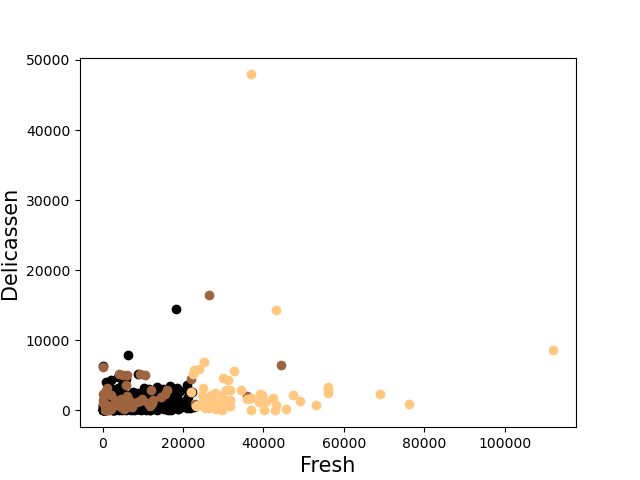
\includegraphics[width = 1.5in]{Fresh_Delicassen.png}} &
        %         \subcaptionbox{caption\label{2}}{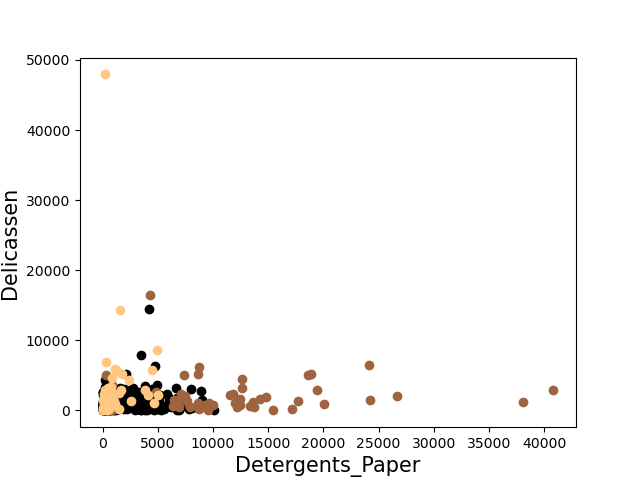
\includegraphics[width = 1.5in]{Detergents_Paper_Delicassen.png}} \\
        %         \subcaptionbox{caption\label{1}}{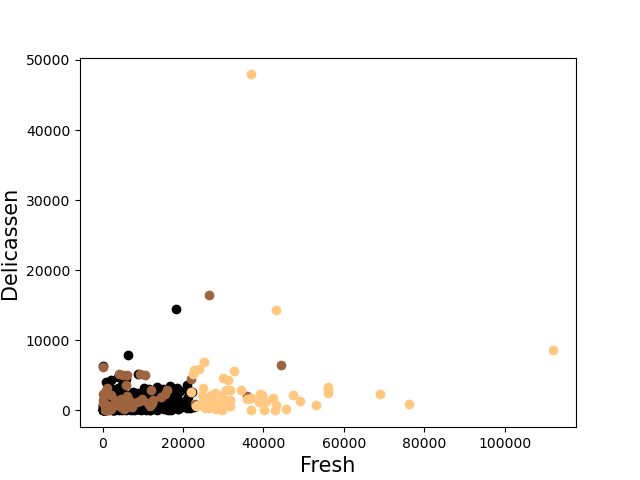
\includegraphics[width = 1.5in]{Fresh_Delicassen.png}} &
        %         \subcaptionbox{caption\label{2}}{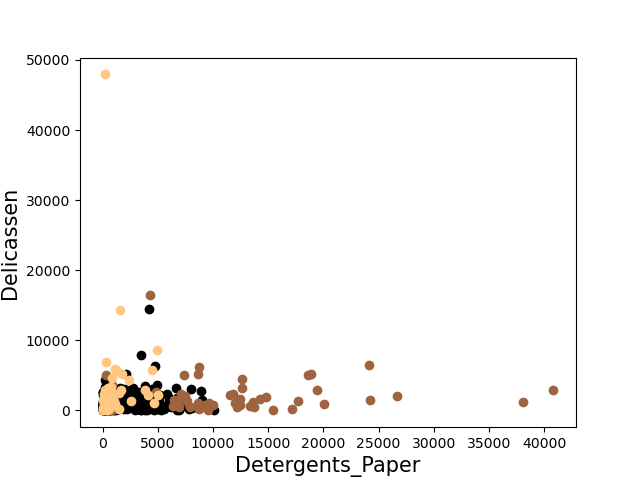
\includegraphics[width = 1.5in]{Detergents_Paper_Delicassen.png}} \\
        %         \subcaptionbox{caption\label{1}}{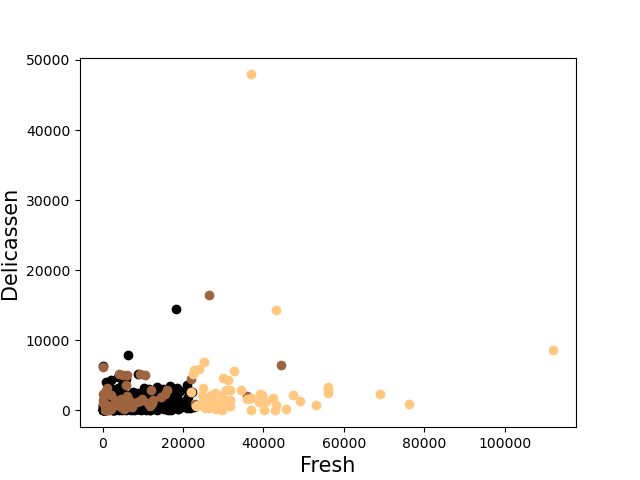
\includegraphics[width = 1.5in]{Fresh_Delicassen.png}} &
        %         \subcaptionbox{caption\label{2}}{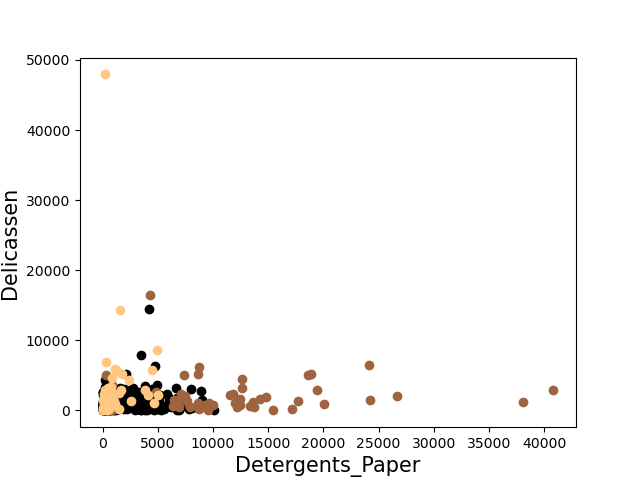
\includegraphics[width = 1.5in]{Detergents_Paper_Delicassen.png}} \\
        %         \subcaptionbox{caption\label{1}}{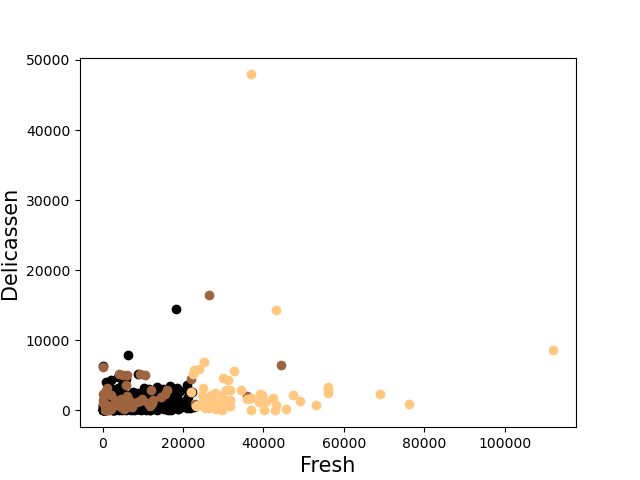
\includegraphics[width = 1.5in]{Fresh_Delicassen.png}} &
        %         \subcaptionbox{caption\label{2}}{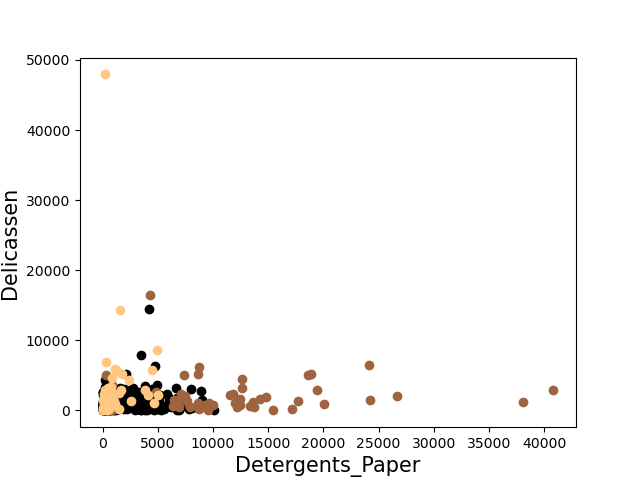
\includegraphics[width = 1.5in]{Detergents_Paper_Delicassen.png}} \\
        %         \subcaptionbox{caption\label{1}}{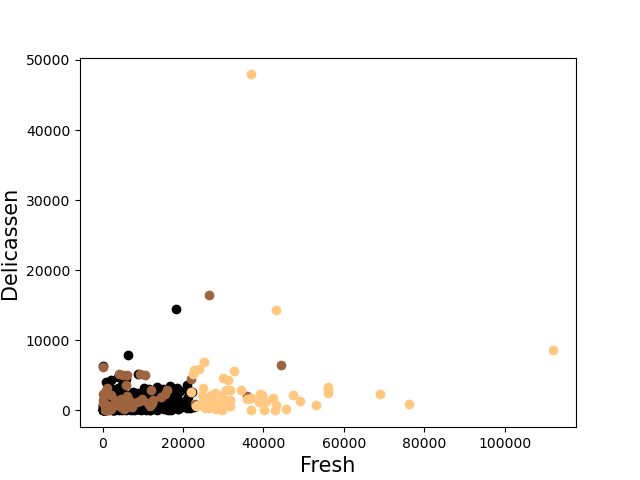
\includegraphics[width = 1.5in]{Fresh_Delicassen.png}} &
        %         \subcaptionbox{caption\label{2}}{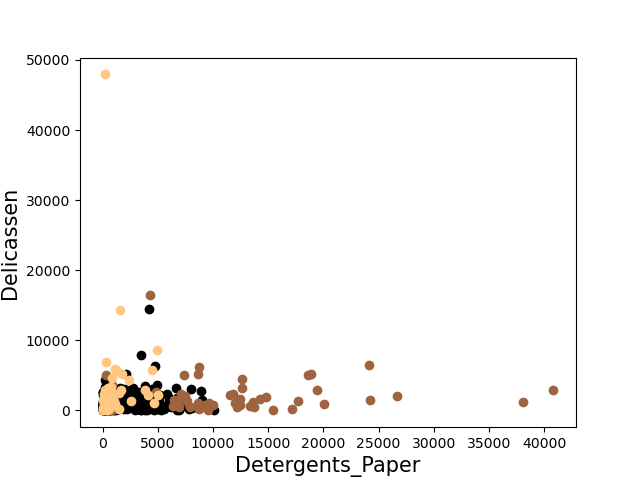
\includegraphics[width = 1.5in]{Detergents_Paper_Delicassen.png}} \\
        %         \end{tabular}
        %         \caption{caption}
        %         \label{3}
        %         \end{figure}





        \begin{figure}
                \begin{tabular}{cccc}
                \subfloat[Fresh vs Delicatessen]{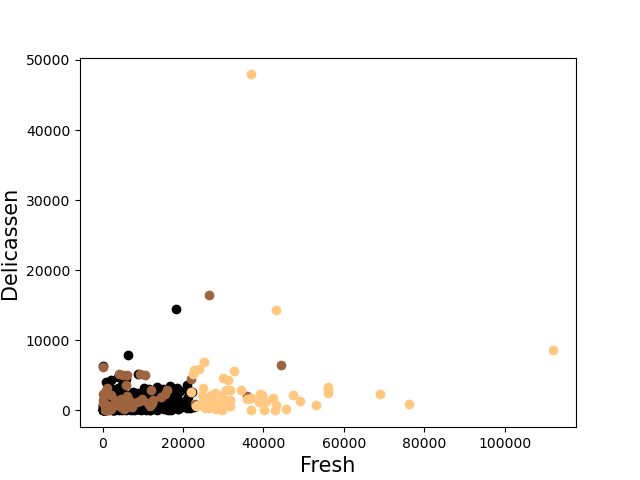
\includegraphics[width = \imWidth]{Fresh_Delicassen.png}} &
                \subfloat[Detergents\/Paper vs Delicassen]{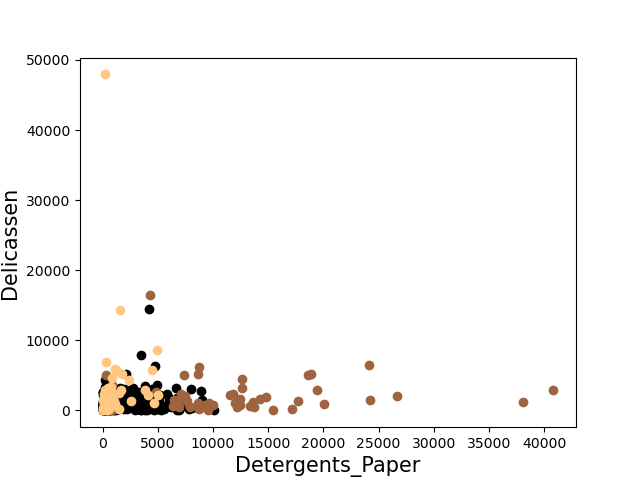
\includegraphics[width = \imWidth]{Detergents_Paper_Delicassen.png}}\\
                \subfloat[Fresh vs Detergents\/Paper]{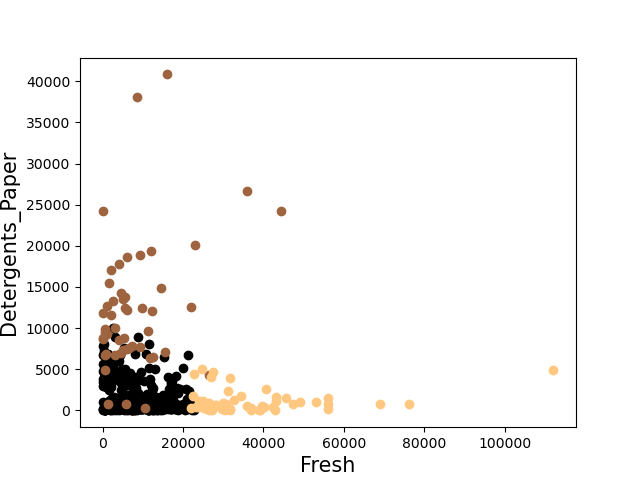
\includegraphics[width = \imWidth]{Fresh_Detergents_Paper.png}} &
                \subfloat[Fresh vs Frozen]{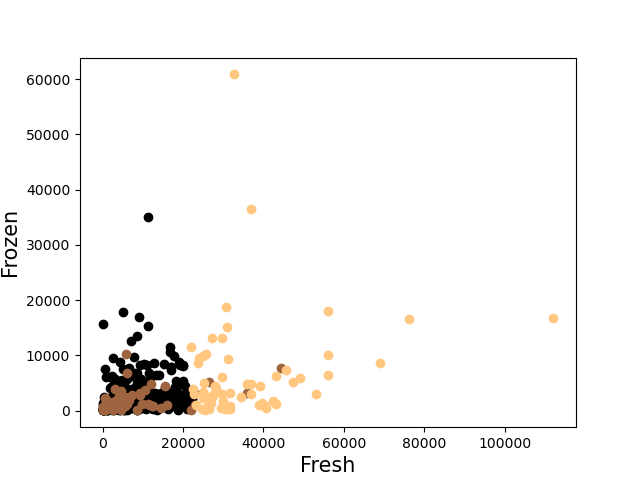
\includegraphics[width = \imWidth]{Fresh_Frozen.png}}\\
                \subfloat[Fresh vs Grocery]{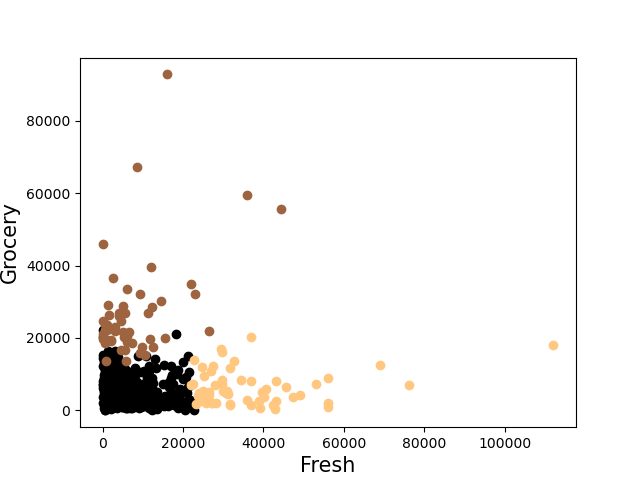
\includegraphics[width = \imWidth]{Fresh_Grocery.png}} &
                \subfloat[Fresh vs Milk]{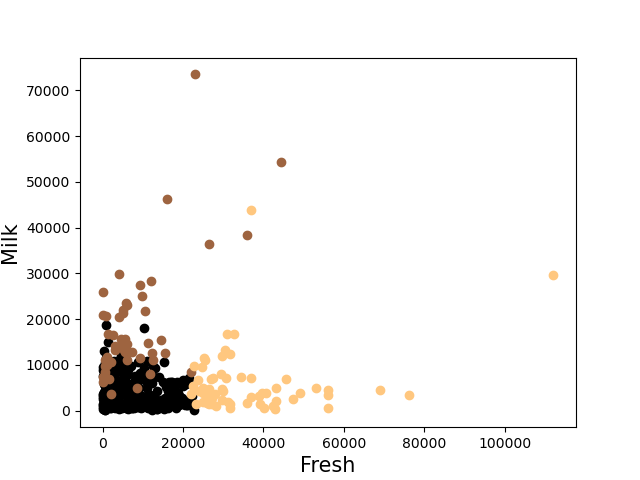
\includegraphics[width = \imWidth]{Fresh_Milk.png}}\\
                \subfloat[Frozen vs Delicatessen]{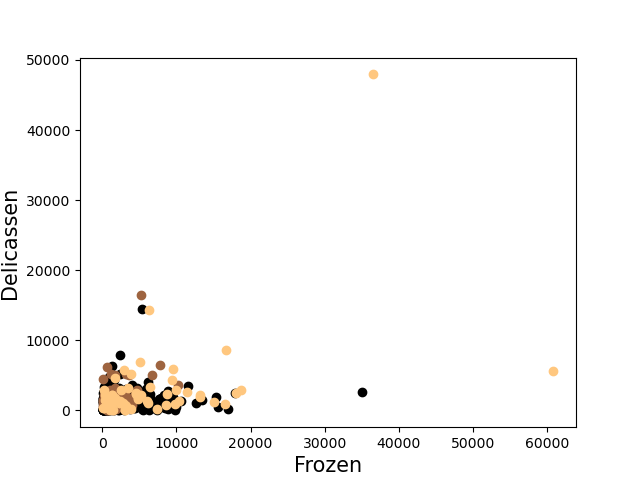
\includegraphics[width = \imWidth]{Frozen_Delicassen.png}} &
                \subfloat[Frozen vs Detergents\/Paper]{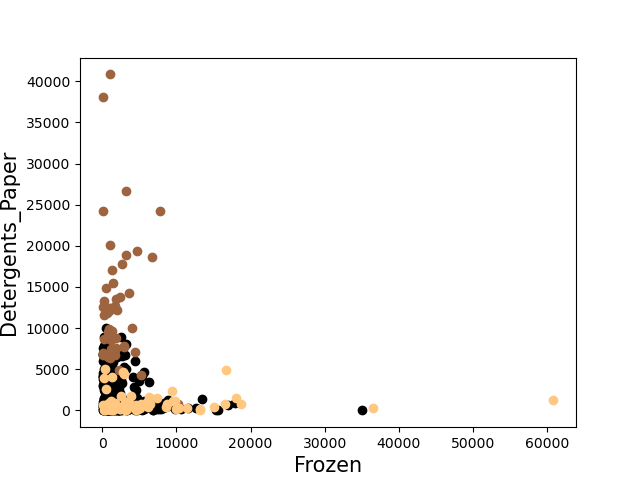
\includegraphics[width = \imWidth]{Frozen_Detergents_Paper.png}}\\
                \subfloat[Grocery vs Delicatessen]{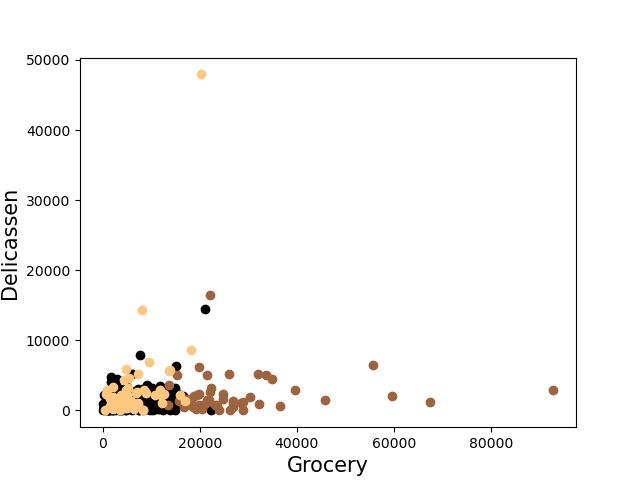
\includegraphics[width = \imWidth]{Grocery_Delicassen.png}} &
                \subfloat[Grocery vs Detergents\/Paper]{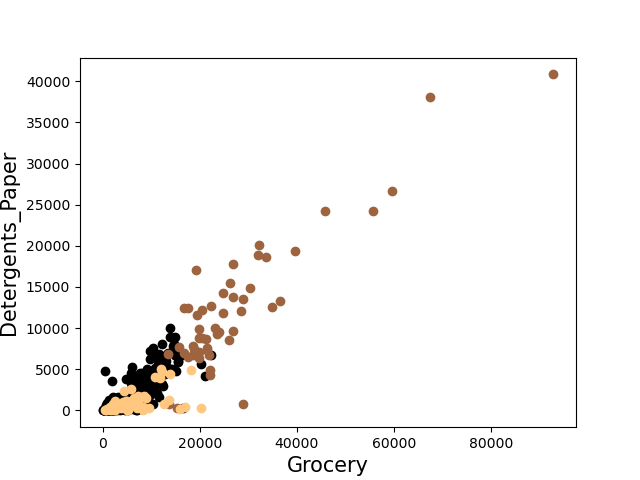
\includegraphics[width = \imWidth]{Grocery_Detergents_Paper.png}}\\
                \subfloat[Grocery vs Frozen]{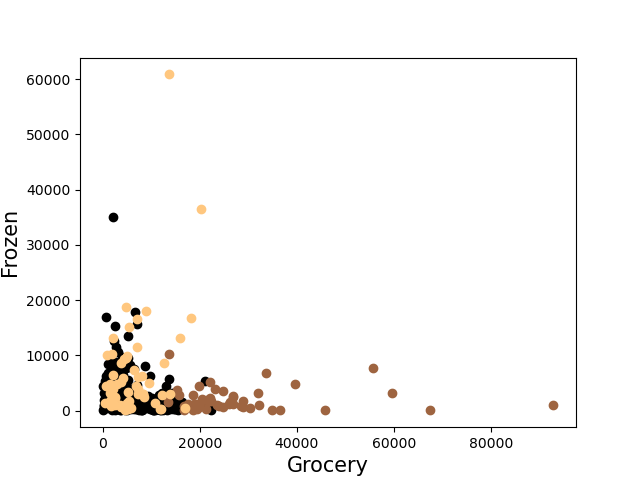
\includegraphics[width = \imWidth]{Grocery_Frozen.png}}&
                \subfloat[Milk vs Delicatessen]{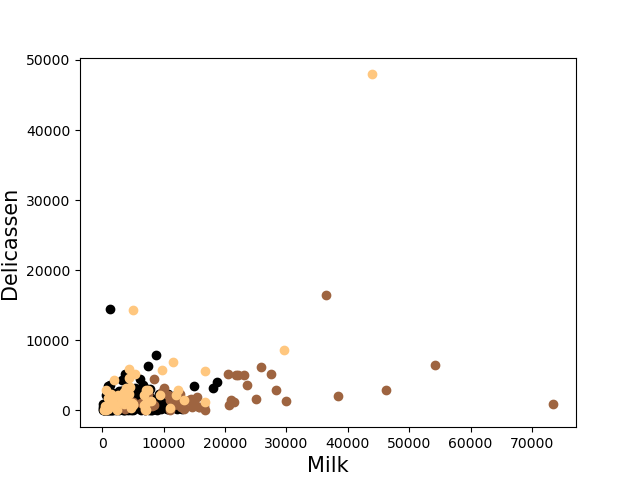
\includegraphics[width = \imWidth]{Milk_Delicassen.png}}\\
                \subfloat[Milk vs Detergents\/Paper]{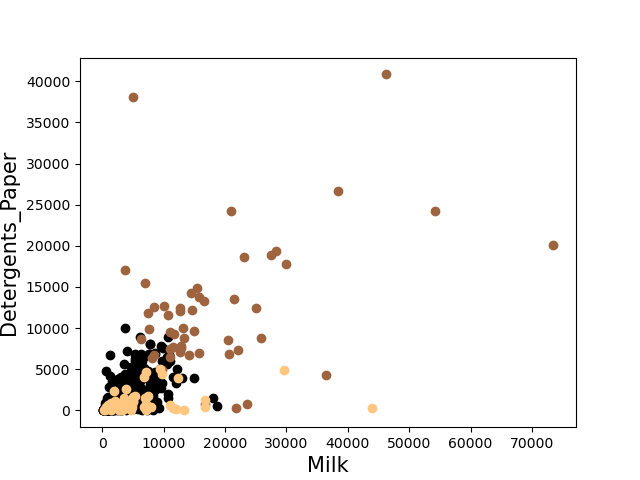
\includegraphics[width = \imWidth]{Milk_Detergents_Paper.png}}&&
                \subfloat[Milk vs Frozen]{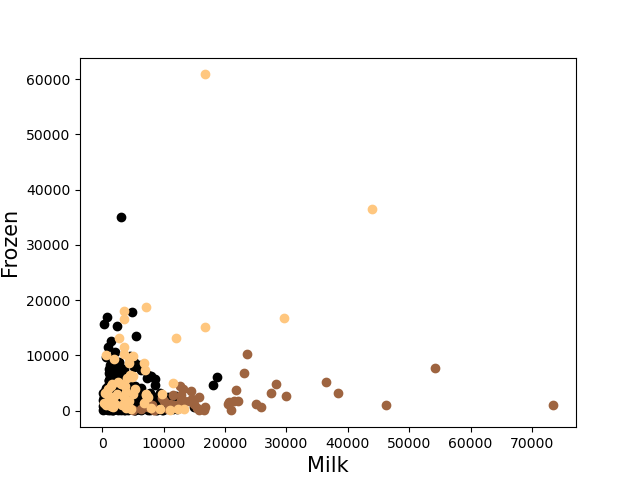
\includegraphics[width = \imWidth]{Milk_Frozen.png}}\\
                \subfloat[Milk vs Grocery]{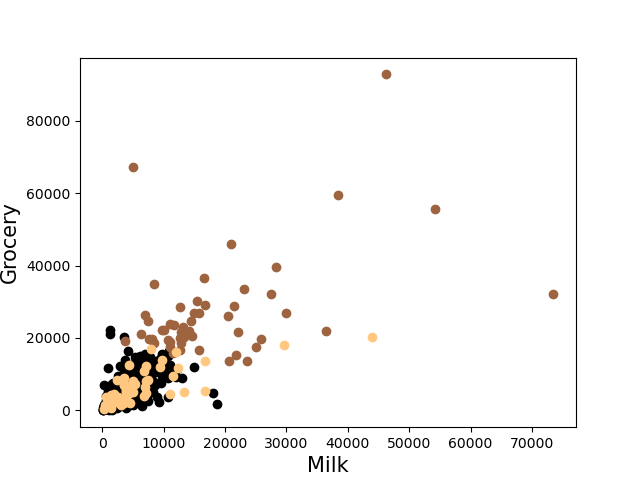
\includegraphics[width = \imWidth]{Milk_Grocery.png}}
                \end{tabular}
                \caption{pairs}
        \end{figure}






% \begin{figure}
%         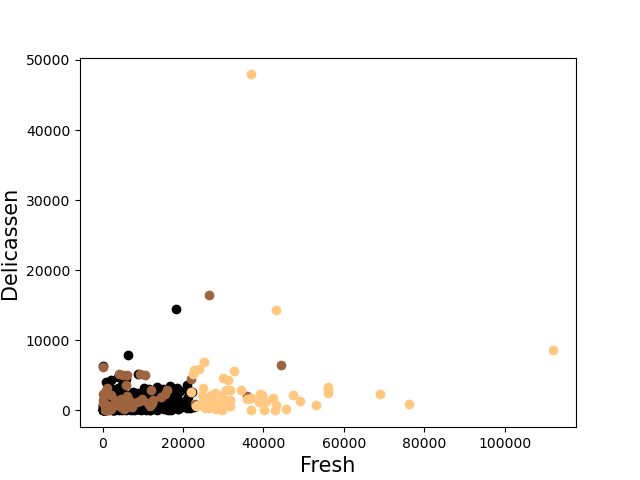
\includegraphics[width=\imWidth]{Fresh_Delicassen.png}
%         \caption{Fresh vs Delicatessen}
%         \caption{fig:freshDel}
% \end{figure}


% \begin{figure}
%         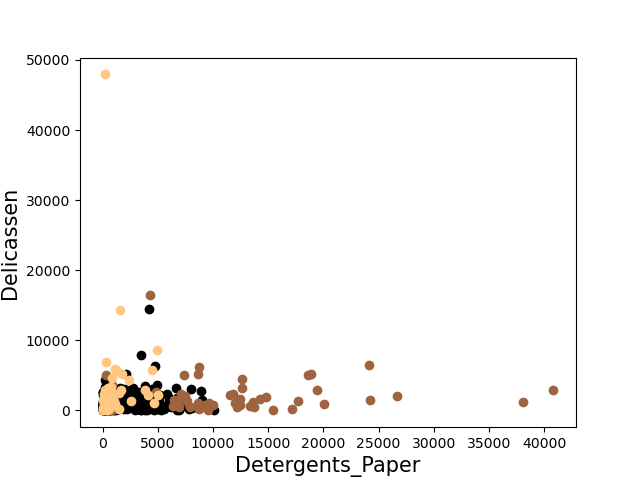
\includegraphics[width=\imWidth]{Detergents_Paper_Delicassen.png}
%         \caption{Fresh vs Delicatessen}
%         \caption{fig:freshDel}
% \end{figure}

% \begin{figure}
%         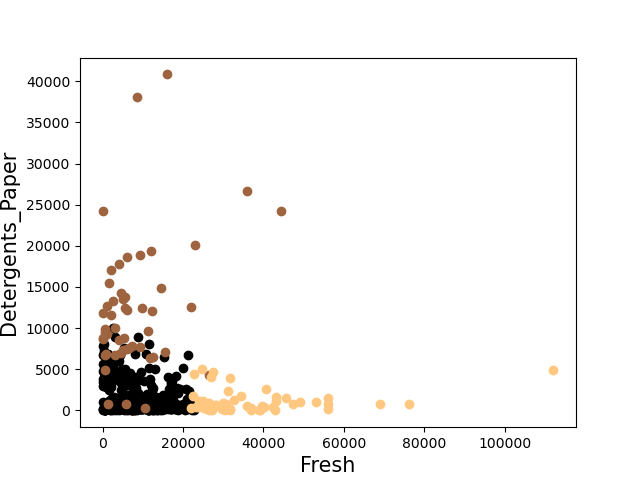
\includegraphics[width=\imWidth]{Fresh_Detergents_Paper.png}
%         \caption{Fresh vs Delicatessen}
%         \caption{fig:freshDel}
% \end{figure}

% \begin{figure}
%         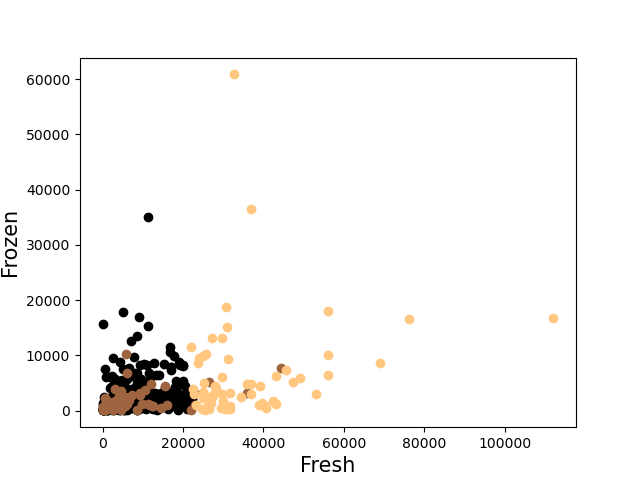
\includegraphics[width=\imWidth]{Fresh_Frozen.png}
%         \caption{Fresh vs Delicatessen}
%         \caption{fig:freshDel}
% \end{figure}

% \begin{figure}
%         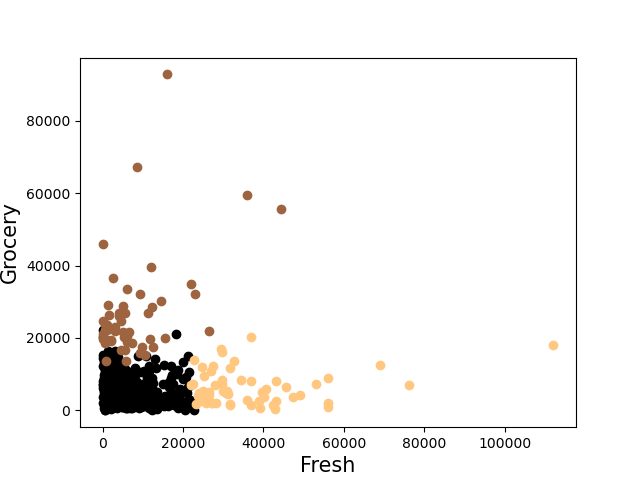
\includegraphics[width=\imWidth]{Fresh_Grocery.png}
%         \caption{Fresh vs Delicatessen}
%         \caption{fig:freshDel}
% \end{figure}

% \begin{figure}
%         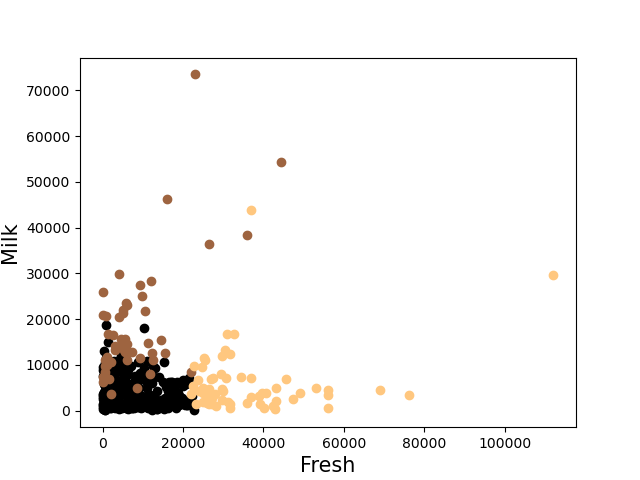
\includegraphics[width=\imWidth]{Fresh_Milk.png}
%         \caption{Fresh vs Delicatessen}
%         \caption{fig:freshDel}
% \end{figure}

% \begin{figure}
%         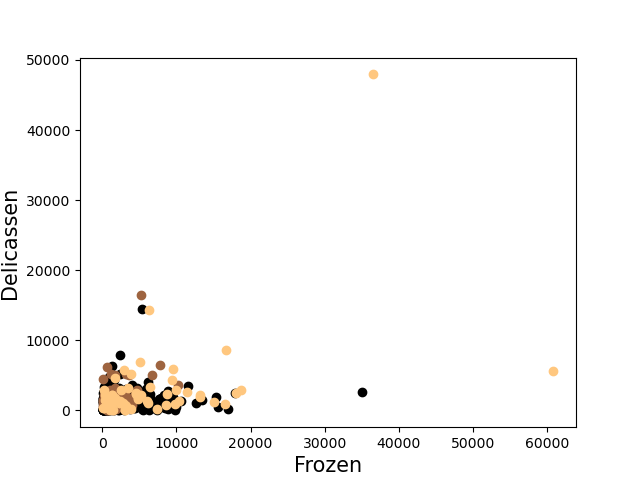
\includegraphics[width=\imWidth]{Frozen_Delicassen.png}
%         \caption{Fresh vs Delicatessen}
%         \caption{fig:freshDel}
% \end{figure}

% \begin{figure}
%         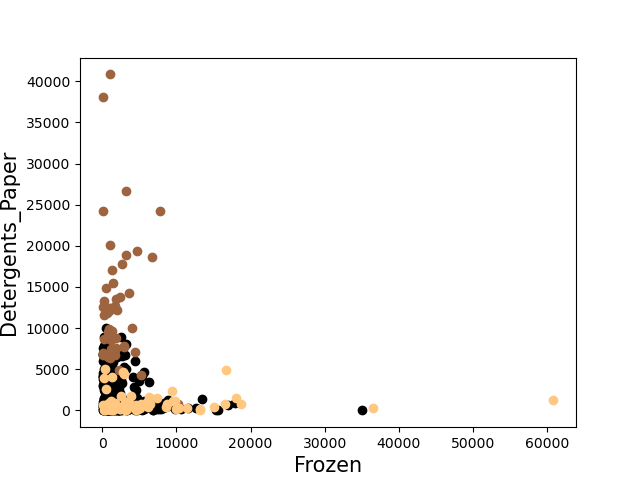
\includegraphics[width=\imWidth]{Frozen_Detergents_Paper.png}
%         \caption{Fresh vs Delicatessen}
%         \caption{fig:freshDel}
% \end{figure}

% \begin{figure}
%         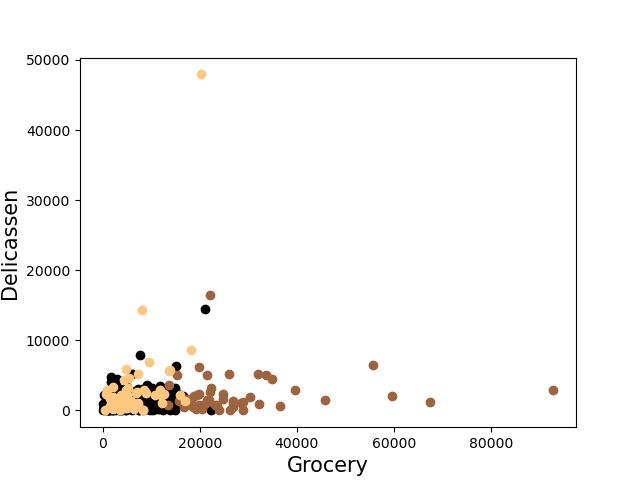
\includegraphics[width=\imWidth]{Grocery_Delicassen.png}
%         \caption{Fresh vs Delicatessen}
%         \caption{fig:freshDel}
% \end{figure}

% \begin{figure}
%         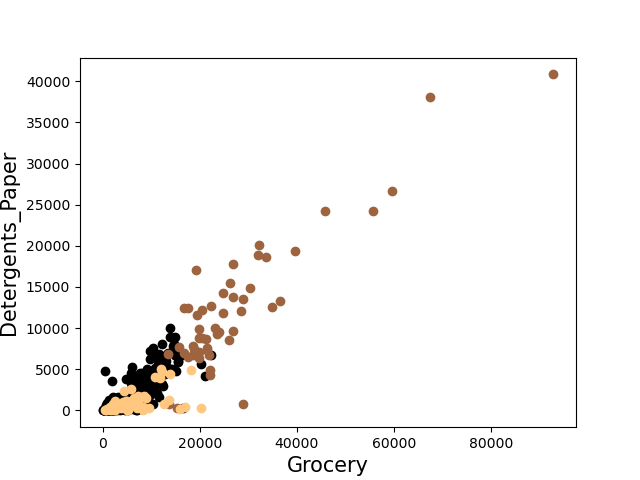
\includegraphics[width=\imWidth]{Grocery_Detergents_Paper.png}
%         \caption{Fresh vs Delicatessen}
%         \caption{fig:freshDel}
% \end{figure}

% \begin{figure}
%         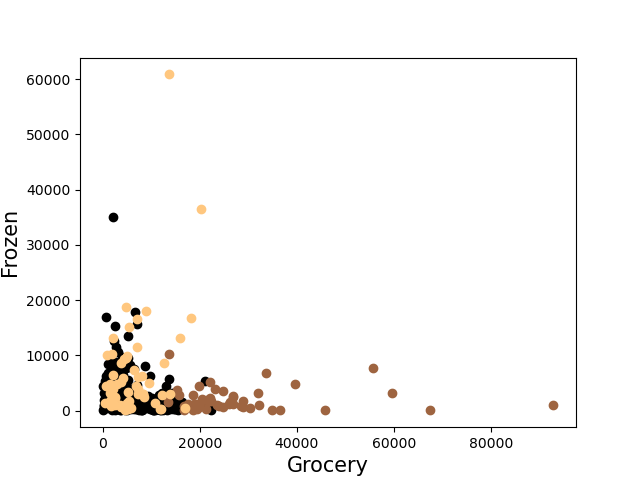
\includegraphics[width=\imWidth]{Grocery_Frozen.png}
%         \caption{Fresh vs Delicatessen}
%         \caption{fig:freshDel}
% \end{figure}

% \begin{figure}
%         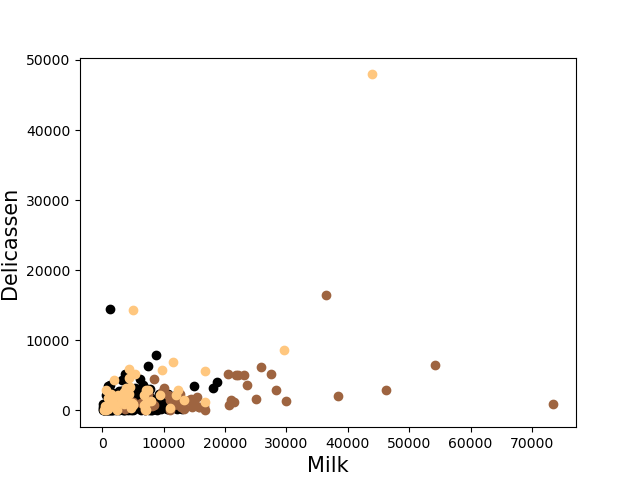
\includegraphics[width=\imWidth]{Milk_Delicassen.png}
%         \caption{Fresh vs Delicatessen}
%         \caption{fig:freshDel}
% \end{figure}

% \begin{figure}
%         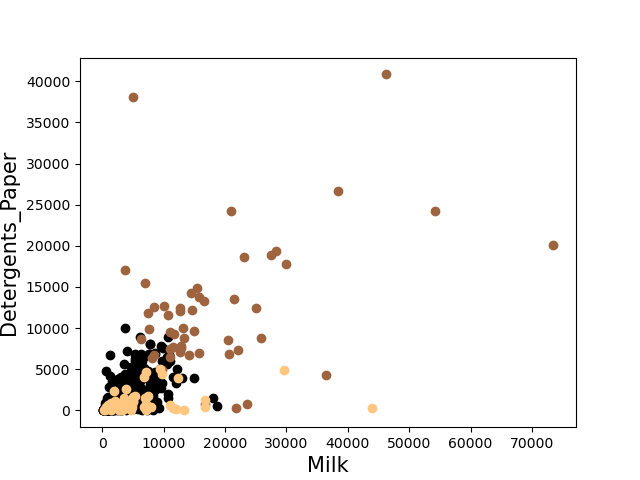
\includegraphics[width=\imWidth]{Milk_Detergents_Paper.png}
%         \caption{Fresh vs Delicatessen}
%         \caption{fig:freshDel}
% \end{figure}

% \begin{figure}
%         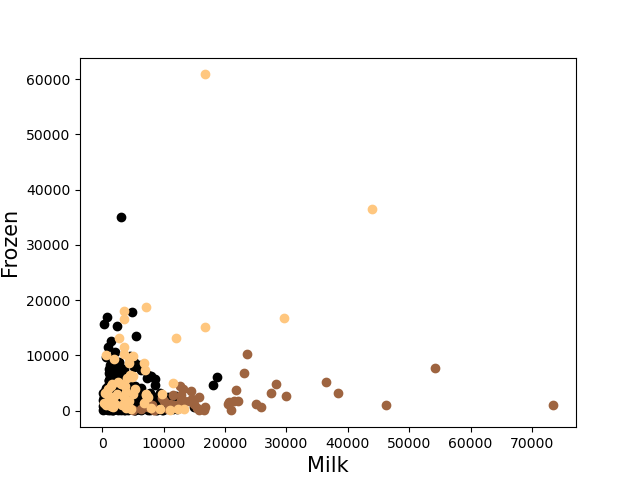
\includegraphics[width=\imWidth]{Milk_Frozen.png}
%         \caption{Fresh vs Delicatessen}
%         \caption{fig:freshDel}
% \end{figure}

% \begin{figure}
%         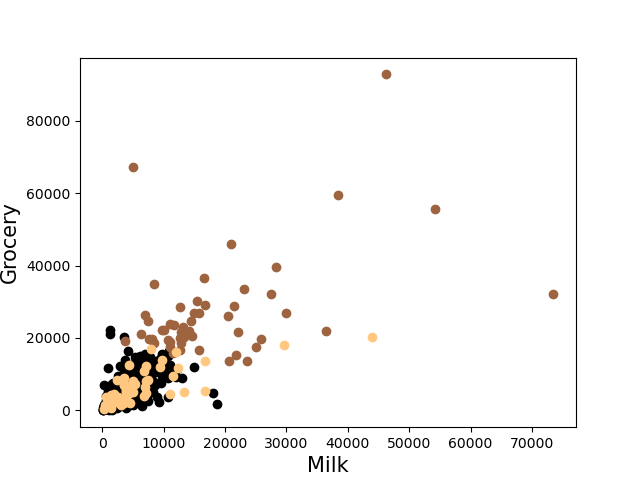
\includegraphics[width=\imWidth]{Milk_Grocery.png}
%         \caption{Fresh vs Delicatessen}
%         \caption{fig:freshDel}
% \end{figure}









*** scatterplots****

It should be noted that some pairwise attributes are better at separating the data than others, when using three clusters. In
several of the scatterplots, the clusters overlap significantly, with little observable distinction between them. For example in
the 'Frozen vs Delicatessen' plot, without the differentiation by the group colours, it would be impossible to tell by visual
observation which datapoints belonged to which cluster. If the dimensionality of the entire dataset were to be reduced for 
simplification, it would make sense to keep only one attribute in this pair. The same can be said for the majority of the pairs.
In fact, the only pairs with much visually observable distinction betweeen clusters are 'Fresh vs Grocery', 'Fresh vs Milk',
'Grocery vs Detergents/Paper', and still this observation is subjective. \\

There is a strong linear correlation between Detergents/Paper and Grocery, suggesting an increase in one of these attributes
would be observed with a rise in the other. A less strong, but still present, linear relationship exists with Milk and Grocery, 
and Milk and Detergents/Paper.\\ 

For many of the pairs containing Delicatessen, it appears there is inelastic expenditure on Delicatessen, where high expenditure in the
opponent attribute gives little to no rise in expenditure on Delicatessen. For example in the Grocery vs Delicatessen pair, the rise in
expenditure in Grocery yields little growth in expenditure on Delicatessen. Perhaps even stronger examples are the 'Fresh vs Delicatessen',
and 'Detergents/Paper vs Delicatessen pairs. There are some outliers present in the data, though this relationship with Delicatessen to 
other attributes may suggest Delicatessen expenditure is consistent, or not considered a choice, meaning the demand for Delicatessen is 
more inelastic, despite always being low.\\


\subsection{Cluster Evaluation} 

\noindent This section contains the cluster evaluation for different values of k in the K-means calculation. The three values of k to be evaluated
are the set \{3,5,10\}. As part of the cluster evaluation, the between-cluster score is calculated. This measures the separation of the clusters from one-another.
This will return a high value if the clusters are separated well.The within-cluster score was also calculated. This is a measure of the cluster density, which, for good clusters, should be high.\\
To compare the clustering between these different k values, the ratio of between-cluster score to within-cluster score was calculated.\\
The results are shown in Table \ref{table:kvals}, rounded to 3 significant figures.
\vspace{4mm}

{\begin{table}
        \centering
        \label{table:kvals}
        
\begin{tabular}{ c|c|c|c|}
        \cline{2-4} & \multicolumn{3}{|c|}{K-Value}\\
        \cline{2-4} & 3 & 5 & 10\\
        \hline
        \multicolumn{1}{|c|}{BC Scores} & 3132200000 &  25621000000 & 216500000000 \\
        \multicolumn{1}{|c|}{WC Scores} & 80330000000 &  52930000000 &  29650000000\\
        \multicolumn{1}{|c|}{BC/WC Ratio} & 0.03899 & 0.4841 &  7.301\\

        \hline

       \end{tabular}

        \caption{BC,WC and BC/WC Ratios}

\end{table}}




\vspace{4mm}
The BC/WC ratio on its own is a relatively useless metric due to the different k values, so it must be normalised. To do this, the Calinski-Harabasz
index  was used. The Calinski-Harabasz index is a measure of separation and density of clusters. To score highly, the clusters should be well separated and
dense. This index showed the best k-value was 5, with a score of 215. Following this were 3 then 10, with scores of 210 and 206 respectively. \\
The calculated values of this index are shown in Table \ref{table:cali}

\vspace{4mm}


{\begin{table}
        \centering
        \label{table:cali}
\begin{tabular}{ |c||c|c|c|}
        \hline
        Metric & 3 & 5 & 10\\
        \hline
        Calinksi-Harabaz's & 210.1 &  215.06 & 206.17\\
        \hline
       \end{tabular}

\end{table}

\end{document}